\documentclass[12pt, a4paper]{memoir} % for a short document
\usepackage[french,english]{babel}

\usepackage [vscale=0.76,includehead]{geometry}                % See geometry.pdf to learn the layout options. There are lots.
%\geometry{a4paper}                   % ... or a4paper or a5paper or ...
%\geometry{landscape}                % Activate for for rotated page geometry
%\OnehalfSpacing
% \setSingleSpace{1.05}
%\usepackage[parfill]{parskip}    % Activate to begin paragraphs with an empty line rather than an indent


%===================================== packages
\usepackage{lipsum}
\usepackage{graphicx}
\usepackage{amsmath}
\usepackage{fullpage}
\usepackage{mathptmx} % font = times
\usepackage{helvet} % font sf = helvetica
\usepackage[utf8]{inputenc}
\usepackage{relsize}
\usepackage[T1]{fontenc}
\usepackage{tikz}
\usepackage{booktabs}
\usepackage{textcomp}%textquotesingle
\usepackage{multirow}
\usepackage{pgfplots}
\usepackage{url}
\usepackage{footnote}
\usepackage{hyperref}
% MINE

\usepackage{listings}
\usepackage{color}


%============================================
\usetikzlibrary{arrows,shapes,positioning,shadows,trees}
\makesavenoteenv{tabular}
\makesavenoteenv{table}
%==============================================
\def\checkmark{\tikz\fill[scale=0.4](0,.35) -- (.25,0) -- (1,.7) -- (.25,.15) -- cycle;}
%Style des têtes de section, headings, chapitre
\headstyles{komalike}
\nouppercaseheads
\chapterstyle{dash}
\makeevenhead{headings}{\sffamily\thepage}{}{\sffamily\leftmark}
\makeoddhead{headings}{\sffamily\rightmark}{}{\sffamily\thepage}
\makeoddfoot{plain}{}{}{} % Pages chapitre.
\makeheadrule{headings}{\textwidth}{\normalrulethickness}
%\renewcommand{\leftmark}{\thechapter ---}
\renewcommand{\chaptername}{\relax}
\renewcommand{\chaptitlefont}{ \sffamily\bfseries \LARGE}
\renewcommand{\chapnumfont}{ \sffamily\bfseries \LARGE}
\setsecnumdepth{subsection}


% Title page formatting -- do not change!
\pretitle{\HUGE\sffamily \bfseries\begin{center}}
\posttitle{\end{center}}
\preauthor{\LARGE  \sffamily \bfseries\begin{center}}
\postauthor{\par\end{center}}
\newcommand{\jury}[1]{%
\gdef\juryB{#1}}
\newcommand{\juryB}{}
\newcommand{\session}[1]{%
\gdef\sessionB{#1}}
\newcommand{\sessionB}{}
\newcommand{\option}[1]{%
\gdef\optionB{#1}}
\newcommand{\optionB} {}

\renewcommand{\maketitlehookd}{%
\vfill{}  \large\par\noindent
\begin{center}\juryB \bigskip\sessionB\end{center}
\vspace{-1.5cm}}
\renewcommand{\maketitlehooka}{%
\vspace{-1.5cm}\noindent
\includegraphics[height=12ex]{pics/logo-uga.png}\hfill\raisebox{2ex}{
\includegraphics[height=14ex]{pics/logoINP.png}}\\
\bigskip
\begin{center} \large
Master of Science in Informatics at Grenoble \\
Master Informatique \\
Specialization \optionB  \end{center}\vfill}
% =======================End of title page formatting

\option{Graphics, Vision and Robotics}
\title{Procedural Stylization} %\\\vspace{-1ex}\rule{10ex}{0.5pt} \\sub-title}
\author{Isnel Maxime}
\date{June 2019} % Delete this line to display the current date
\jury{
Research project performed at MAVERICK \\\medskip
Under the supervision of:\\
Romain Vergne\\
Joëlle Thollot\\\medskip
Defended before a jury composed of:\\
Head of the jury\\
Jury member 1\\
Jury member 2\\
}
\session{June \hfill 2019}
\setcounter{tocdepth}{4}
\setcounter{secnumdepth}{4}

%%% BEGIN DOCUMENT
\begin{document}

\selectlanguage{English} % french si rapport en français
\frontmatter
\begin{titlingpage}
\maketitle
\end{titlingpage}

%\small
\setlength{\parskip}{-1pt plus 1pt}

\renewcommand{\abstracttextfont}{\normalfont}
\abstractintoc
\begin{abstract}
Your abstract goes here...
\end{abstract}
\abstractintoc

\renewcommand\abstractname{Acknowledgement}
\begin{abstract}

    %I would first like to thank my internship advisors, Fabrice Neyret, for his valuableinsight on procedural texturing and comprehension of artifacts, Joelle Thollot,who never failed keeping this project on schedule, while sharing her knowledgeabout non-photorealistic rendering, and Romain Vergne, who successfully steeredmy research about perception the right way while proofreading this work.I would also like to thank the entire MAVERICK team for their warm welcome,as I felt integrated since the very first days, and it would be a pleasure to keepworking along them, maybe for a PhD.I would like to thank Inria and the Laboratoire Jean Kuntzmann for providing mewith the necessary resources to carry out this work.Finally, I would like to thank James Crowley for allowing me to defend this researchproject alongside other students of the MoSIG master, even though I am followingan ISI specialization at Ensimag.

I would like to express my sincere gratitude to .. for his invaluable assistance and comments in reviewing this report...
Good luck :)
\end{abstract}


\renewcommand\abstractname{R\'esum\'e}
\begin{abstract} \selectlanguage{French}
Your abstract in French goes here...
\end{abstract}
\selectlanguage{English}

\cleardoublepage

\tableofcontents* % the asterisk means that the table of contents itself isn't put into the ToC
\normalsize

\mainmatter
\SingleSpace
%==============================CHAPTERS==================
\chapter{Introduction}


\section{Background}

\section{Problem Statement}

A part of the computer graphics is create non-photorealistic images. A method to do this is to stylize 3D objects and 3D scenes. Stylize an object means create an image that imitates the style of an artist who would have drawn it on sheet of paper. There exist many different styles like hand drawing, brush painting, pointillism painting, stippling, watercolor painting, etc.

The main problem of stylizing a 3D object in an animation is the \textit{temporal coherence}. The \textit{temporal coherence} problem in non-photorealistic rendering encompasses both spatial and temporal aspects of the marks. The effect given by the stylization has to be kept if the object is moving, rotating and scaling. Many research has been done to solve this problem of \textit{temporal coherence} \cite{vergne_implicit_2011, benard_dynamic_2009, bleron_motion-coherent_2018}. Bénard et al. separate this problem is three sections inspired by previous work\cite{meier_painterly_1996, cunzi_dynamic_nodate, breslav_dynamic_nodate, benard_state---art_2011} the ideal solution (Figure \ref{problem_temporal_coherence} a) could correspond to something drawn by an artist at each frame. Neglect one of this three goals provide artifacts (Figure \ref{problem_temporal_coherence} b-d).

\begin{figure}
    \begin{center}
    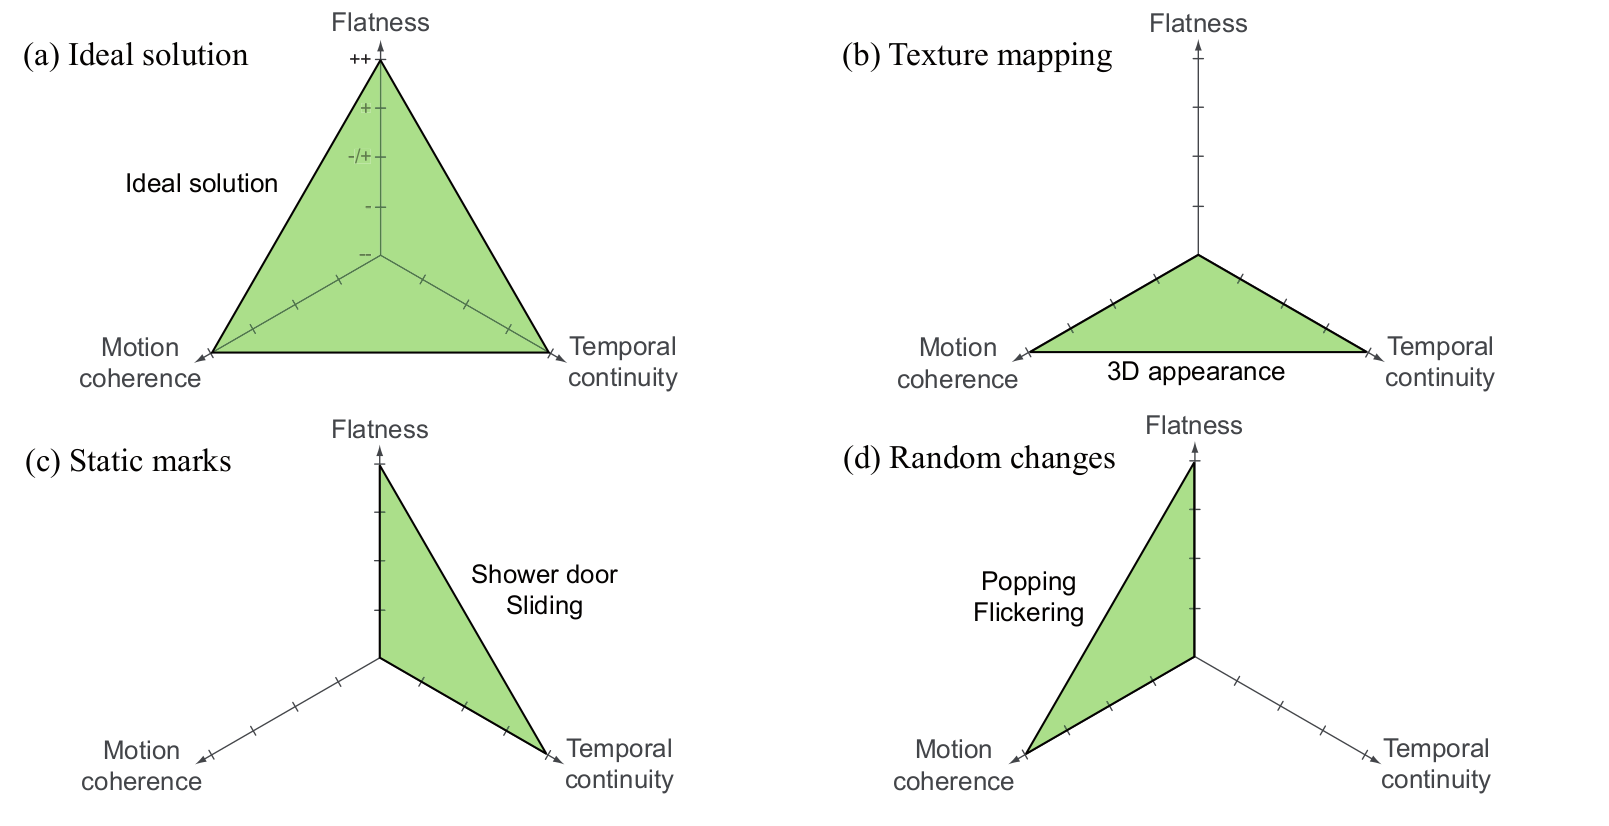
\includegraphics[scale=0.3]{pics/temporal_coherence.png}
    \end{center}
    \caption{Problem involve by temporal coherence depending of the flatness, temporal continuity, motion coherence.}
    \label{problem_temporal_coherence}
\end{figure}

\subsection{Flatness}

The impression of drawing on a flat surface gives the \textit{flatness}. The stylization has a good \textit{flatness} if the image rendered has a good 2D appearance. In order to keep this effect, the size and the distribution of the marks of your stylization have to be independent of the distance between the stylized object and the camera.

\subsection{Motion Coherence}

\textit{Motion coherence} is a correlation between the motion of marks and the motion of the 3D object. Bad \textit{Motion coherence} will give the impression to see the scene through a semi-transparent layer of marks, this is called \textit{shower door} effect \cite{meier_painterly_1996}, an example to illustrate what happens when there is a bad \textit{Motion coherence} is the movie \textit{Loving Vincent}\cite{LovingVincent}. The goal is to provide in 2D screen space a perceptual impression of motion as
close as possible to the 3D displacement in object space.

\subsection{Temporal continuity}

\textit{Temporal continuity} is the quality of minimizing changes from frame to frame to ensure fluid animations. In order to have good \textit{temporal continuity}, the marks of the image have to fade slowly during the animation. Human perception is very sensitive to \textit{temporal incoherence} according to some perceptual studies\cite{percept_studies, Schwarz_2009}. \newline


The problem introduced in the works of Bénard et al.\cite{benard_state---art_2011} is the difficulty to have a ideal solution, the one that has a good \textit{flatness}, a good \textit{motion coherence} and a good \textit{temporal continuity}. These three goals are inherently contradictory when you improve one you neglect one or maybe more. So researchers work to find solutions that make \textit{trade-offs} between these three goals. Our solution is a \textit{trade-offs} too.

\section{Scientific approach}

\section{Contents of this report}

\chapter{Previous Work}



The problem of stylizing a 3D object has received many attention in previous work. There are many methods to stylize. Each of these method have their advantages and disadvantages about the temporal coherence. We separated these ways to stylized in four differents sections.


\section{Image Space}

This simpliest way to stylize a 3D model is to do in image space. The scene is rendered as an image in a texture and from this image the stylization can proceed.
The idea is from this image succeed to compute at each pixel the right color of the splat if this is stroke based rendering or which color of an external texture have to be put on this pixel.
To do an initial painting with strokes Hertzmann's [Image and Video-Based Artistic Stylisation, 2013] add strokes colored depending on the image in the image and decide to delete or replace it to fit at best curves to edges of the image.
Implicit Brushes for Stylized Line-based Rendering [R.Vergne, 2011] use convolution of points to have an hand drawing effect. These points are placed depending on the \textit{feature profile} which is extracted from the image using maximum of the luminance gradient and the DeCarlo algorithm.
\section{Object Space}

\section{Texture Mapping}

\section{Stroke Based}

\chapter{Realisation}


\section{Overview}

\begin{figure}[H]
    \begin{center}
    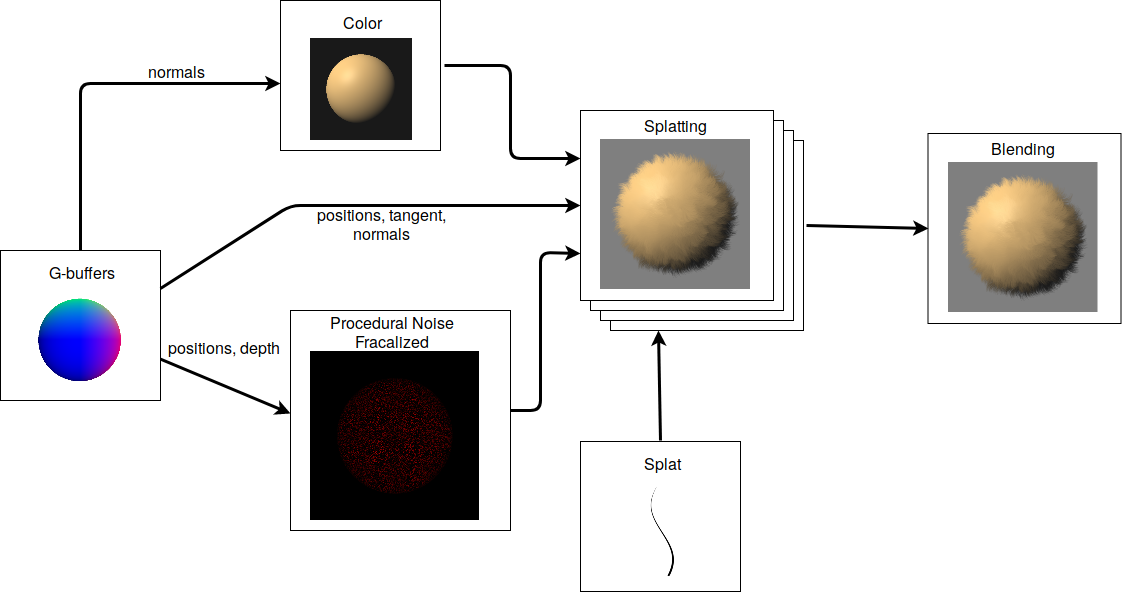
\includegraphics[scale=0.4]{images/Overview2.png}
    \end{center}
    \caption{Overview of our solution.}
    \label{overview}
\end{figure}

As explained in the state of the art and in the figure\ref{tableau_comparatif} each approach has its advantages and its disadvantages. Our main idea is to use procedural texture rendered in the object space to guide the splats in image space.  This solution permits to apply something like 2D images on the screen so have a good \textit{flatness} while keeping the information on the silhouettes, the orientation, the depth, etc. This solution only needs images as input so it can easily be integrated into most of rendering pipelines without re-rendered images. In the figure \ref{overview}, there is an overview of our pipeline. First we computed all the data  in what we called G-Buffer (normals, tangents, position, matrices, depth, UV coordinates) then we render a color (in this example a simple shading) after this we computed our procedural noise that will help to anchor the splats to the object and we choose the splat that will convolves in order to make the stylization. Finally, we draw splat on the entire screen, then we decide which one has to be displayed this is the splatting step and the last step is the blending which computed which splat is in front of the others and which color has to be prompted. \newline

We chose to use mark based methods to stylize our scene because texture-based methods in image space give a poor variety of styles as said in the work of Bénard et al.\cite{benard_dynamic_2009}. This mark-based method implies to decide where in the image the splats will be drawn. In our problem, the goal is to anchor these splats with the objects in order to have the same motion for the splats and the object. This avoid the problem of \textit{shower door effect} and ensure good \textit{motion coherence}. So we needed anchor points depending on the position of our object. Therefore in our approach, we used a procedural noise\cite{perlin_improving_2002} as a texture our 3D object. The procedural noises are easy to implement, fast to compute and easy to manipulate. Like every texture computed in object space, it has a good motion coherence.


\section{Procedural noise and fractalization}

\begin{figure}[H]
    \begin{center}
    
\includegraphics[width=40mm, height=40mm]{images/PerlinNoise2d.png}
    
\includegraphics[width=40mm, height=40mm]{images/GaborNoise2d.png}
    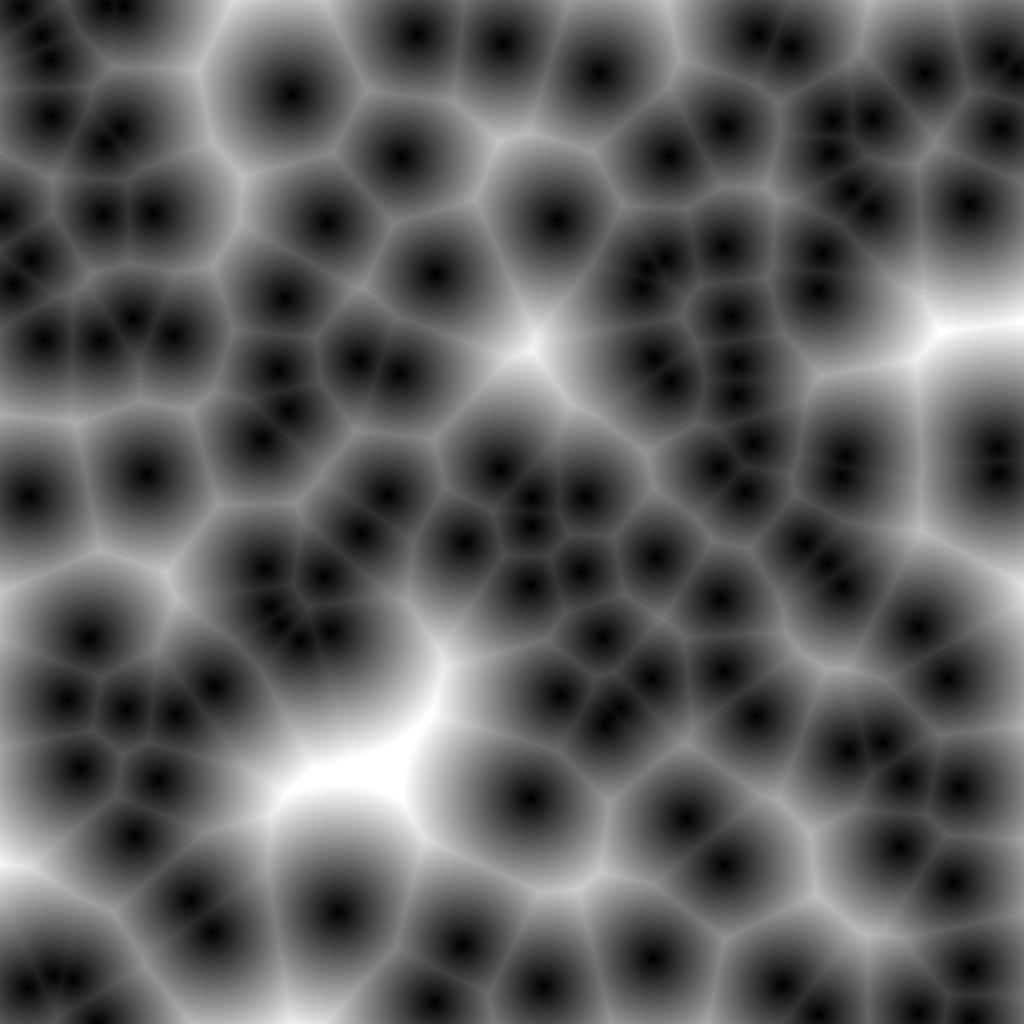
\includegraphics[width=40mm, height=40mm]{images/WorleyNoise2d.jpg}
    \end{center}
    \caption{Examples of procedural texture: \textit{left using perlin noise, middle using Gabor noise,right using worley noise}.}
    \label{procedural_texture}
\end{figure}

% Description of procedural noise

We compute procedural texture in order to create anchor points. In computer graphics, they are usually used to create more complex rendering like the marble texture (figure \ref{marble_rendering}). These textures are computed from procedural noise with a mathematical process with only the position as a parameter. The algorithm to create these textures are implicit that means that with only one position you can have the value without knowing the rest of the texture. That is why they are very used is computer graphics because they can be computed in parallel on GPU. There exist much procedural noises such as Perlin noise, Worley noise, Gabor noise, Value noise, Gradient noise, etc. In order to map the procedural texture to the 3d object, we compute it with the vector position of each vertex of the object.

% how we use it

\begin{figure}[H]
    \begin{center}
    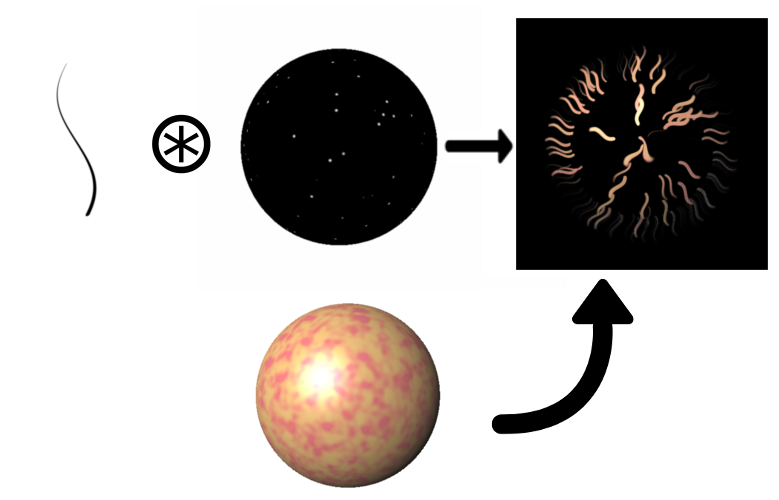
\includegraphics[scale=0.6]{images/noise/addition.png}
    \end{center}
    \caption{Usage of procedural texture to anchor splats: (left: splat image, middle: procedural teture, right: rendered image, bottom: color).}
    \label{procedural_noise_anchor}
\end{figure}

In our case, we used the procedural texture to anchor the splat. For each pixel of the final image we "paste" a splat. Each splat as a weight that will correspond to its opacity during the splatting and the blending. The value of this weight corresponds to the value of the noise on the current point. In the figure \ref{procedural_noise_anchor}, you can see in the areas where the noise is close to zero there is no splat displayed in the final image. Thanks to this mechanism we can control the density of splat in the image. In our case, we worked mainly with the Worley that when inverted almost correspond to point distribution.



% Worley

\begin{figure}[H]
    \begin{center}
    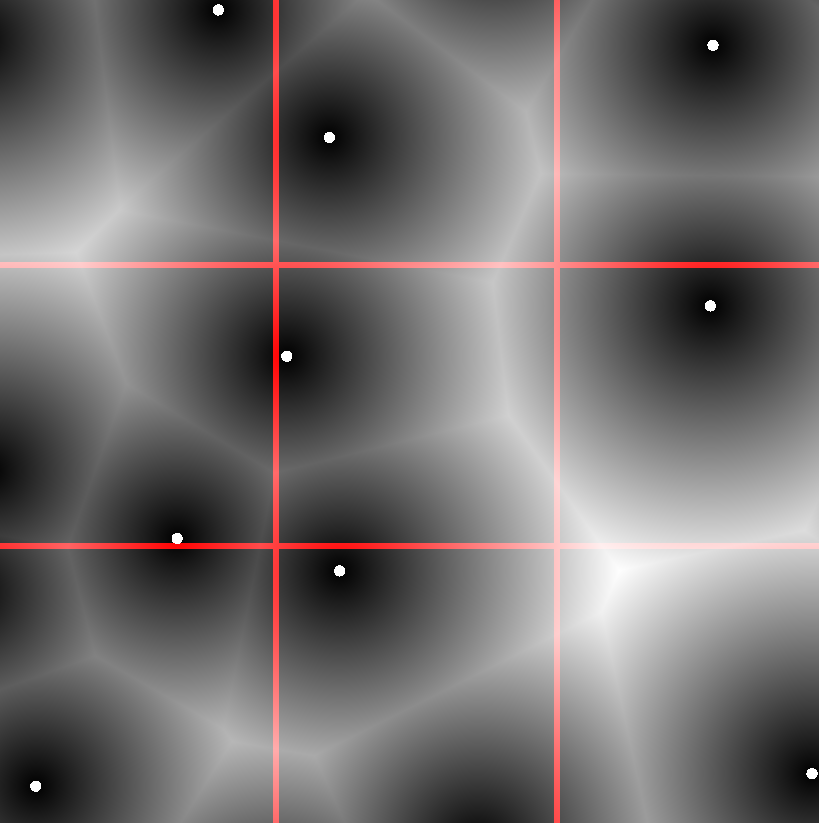
\includegraphics[scale=0.2]{images/noise/worley_explain.png}
    \end{center}
    \caption{Worley noise in 2d.}
    \label{worley_explain}
\end{figure}

We mainly work with the Worley noise which is a cellular noise as you can see at the right in the figure \ref{procedural_texture}. To create a procedural texture from a Worley noise, we divide the image in cells (squares with the same size in 2d, red lines in the figure \ref{worley_explain}), then in each square we compute a point with a seeded random (white dot in the figure \ref{worley_explain}) and finally at each pixel of the texture we put as value the distance with the closest point computed previously with the random seed. Increase the frequency of this noise correspond to divide the image with smaller cells and so have more cells in the image. We explained the principle for a 2d texture but it is the same principle in 3d with a volumic grid. In our pipeline, we use the inverse of this noise (1-worleynoise) in order to have the white pixels of the procedural texture as anchor points. We add a threshold parameter to compute the noise in order to reduce the number of splat to display but especially to have small points in the procedural texture if not the splats convolve as you can see in the rendered image in the figure \ref{procedural_noise_anchor}.

\begin{figure}[H]
    \begin{center}
    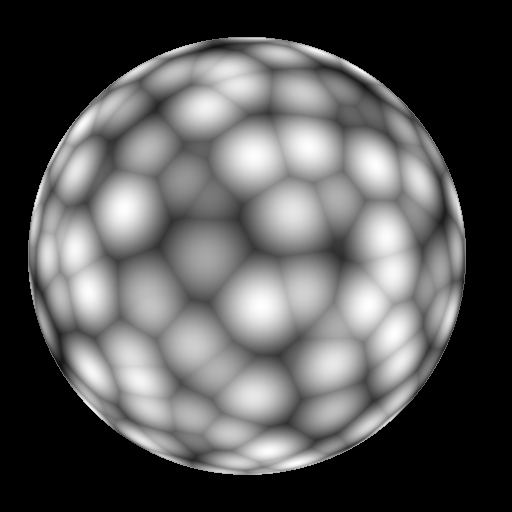
\includegraphics[scale=0.3]{images/noise/worley3d_thresh_1.png}
    
\includegraphics[scale=0.3]{images/noise/worley3d_thresh_2.png}
    
\includegraphics[scale=0.3]{images/noise/worley3d_thresh_3.png}
    \end{center}
    \caption{Use of threshold in the case of Worley noise with the same frequency.}
    \label{worley_threshold}
\end{figure}

As we said before we use a threshold for the purpose of having another control on the noise. With the Worley noise, this threshold corresponds to the "size" of the points. If we increase the threshold the points become smaller as you can see in the figure \ref{worley_threshold}. In order to facilitate the control of this noise, we adapt this threshold according to the frequency and the distance from the camera. That means that the size of each point is constant if the frequency or/and the distance from the camera is changed. \newline

% Add fractalization


\textbf{Fractalization}

\begin{figure}[H]
    \begin{center}
    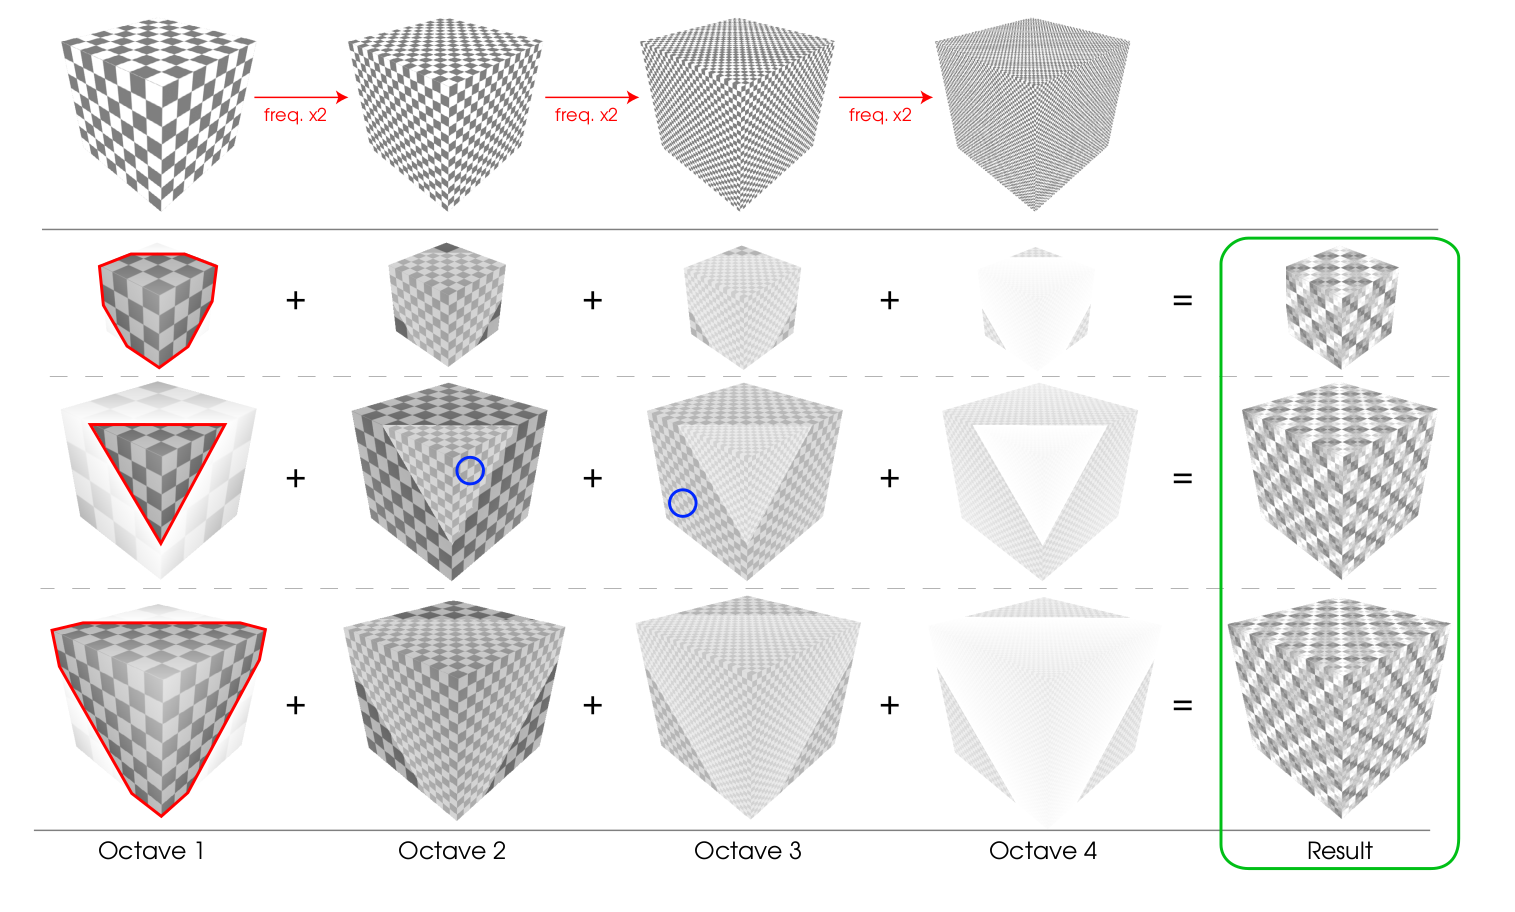
\includegraphics[scale=0.3]{images/fractalization_principle.png}
    \end{center}
    \caption{Principle of fractalization \cite{benard_dynamic_2010}.}
    \label{fractalization_principle}
\end{figure}

\begin{figure}[H]
    \begin{center}
    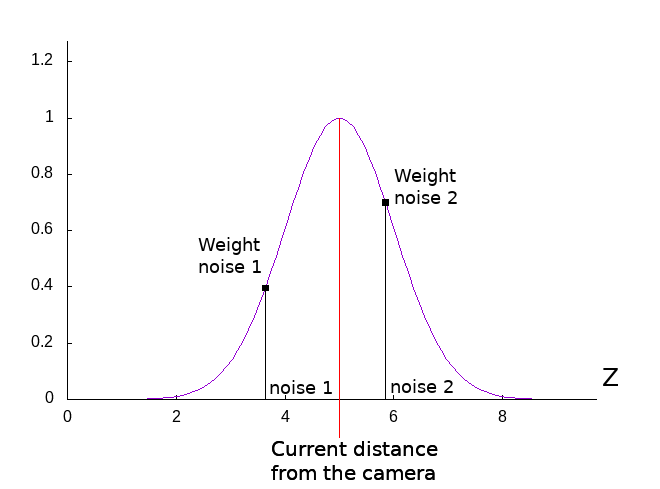
\includegraphics[scale=0.6]{images/fractal_explained.png}
    \end{center}
    \caption{Combination of the noises with the weight value in this case with 2 noises.}
    \label{fractalization_practical}
\end{figure}


Bénard et \textit{al.}\cite{benard_dynamic_2010} introduce the mechanism of fractalization on textures. This technique creates an impression of infinite zoom effect (like in this example: \href{https://www.shadertoy.com/view/XlBXWw?fbclid=IwAR1fU2JxQzXtks1ZcmVmzrHiv646G8w2gWceeiV-UToeFkAFMQ2NecbsGGs}{ShaderToy of Neyret Fabrice}). This is helpful in our case because when the camera is getting closer and closer or further and further less or more points in the texture. With this mechanism, we can get a quasi-constant number of points on the screen. In our method of stylizing it improves the \textit{temporal continuity} because there is always display even if you get very close to the object and it also improves the \textit{flatness} impression because there is almost the same number of anchor points in the screen and their size is quasi-constant. This method alters the original pattern of the texture as you can see in the figure \ref{fractalization_principle} it can be an issue because some pattern cannot be fractalized (like the checkboard pattern) but it works well with stochastic textures. To creates this fractalization, they use textures at multiple frequencies (not necessary procedural texture) (see figure \ref{fractalization_principle}) and they combine them with the transparency and they overlap them according to the distance from the camera as you can see in the results of the figure \ref{fractalization_principle}. \newline


The figure \ref{fractalization_principle} show 4 noises (octaves) at different frequency it is a zooming cycle. As you can see, if the distance from the camera is close to 0 the frequency of the noises is high and if we move away from the object the frequency decrease. So when the distance from the camera is twice as large the frequency of the noise displayed is multiplied by 2. During the zoom, we modulate each octave with a weight. To compute the weight of each noise we use Gaussian interpolation centered on our current distance from the camera (see figure \ref{fractalization_practical}) with a sigma depending on the number of noises that we want to combine.







 % Bénard et \textit{al.}\cite{benard_dynamic_2010} use the same principle but with procedural textures. They create multiple noises with different frequency and combine them playing with transparency. Moreover, they overlap the noise to make an impression of infinite zoom effect (like in this example: \href{https://www.shadertoy.com/view/XlBXWw?fbclid=IwAR1fU2JxQzXtks1ZcmVmzrHiv646G8w2gWceeiV-UToeFkAFMQ2NecbsGGs}{ShaderToy}). With this method patterns of the texture have an almost constant size regardless of the size of the object but it can create small problems of \textit{temporal continuity}. In our method, we will use this technique of fractalization of a procedural noise. \newline

\section{Splatting}

\begin{figure}[H]
    \begin{center}
    \fbox{
\includegraphics[width=30mm, height=30mm]{images/splats/dot_splat.png}}
    \fbox{
\includegraphics[width=30mm, height=30mm]{images/splats/hair_splat.png}}
    \fbox{
\includegraphics[width=30mm, height=30mm]{images/splats/line_splat.png}}
    \fbox{
\includegraphics[width=30mm, height=30mm]{images/splats/paint_splat.png}}
    \end{center}
    \caption{Example of what the splats can be.}
    \label{splat_examples}
\end{figure}

The marks based method try to imitate how the artists do when they stylize. They draw on a flat surface that gives a good impression of \textit{flatness}. We use the same principle to stylize our scene. We put splats/marks directly on the image like an artist will do (illustrated in the figure \ref{procedural_noise_anchor}). \newline

In our solution, the user controls the splat image he can use anything. These marks can be leaves, hairs, dots, feathers, lines, paint brushes, etc. They can also be created from a procedural noise. The user has also the control on the size of these splats, he has global control of the size and control on a specific part of the object through a texture. The rotation of the splats is also a parameter that the user can control. He can choose to rotate all the splat, for example, depending on the normals or depending on the tangents. \newline

Artists control how their marks are combined for example if he is doing painting he could want to have non-transparent marks in order to cover the marks behind the new one. He could want more transparency if for example, he wants to do watercolorization.\newline

In our method, we take this into account during the blending of all marks. The user can control how many marks the stylization will mix and control the transparency (alpha blending). For example, the user can choose to only show the marks at the top of the flat surface (the closest to the camera) or he can choose to mix some marks in order to account some marks covered.


\section{Stylization}

As explained in the previous section, in our method, the user controls the content of the splats, their size, their orientation, the density of splat on the object and how they are blended with the alpha blending. In this section, we will show you some examples of how we did specific style using our pipeline. \newline

\textbf{Pointillism}

\begin{figure}[H]
    \begin{center}
    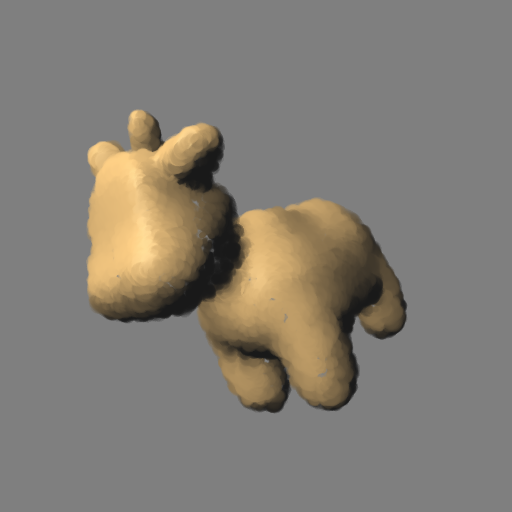
\includegraphics[width=80mm, height=80mm]{Resultats/spotPoint/final.png}
    \end{center}
    \caption{Example of pointillism with our method.}
    \label{final_point}
\end{figure}

In order to make pointillism style we use a dot as splat (gaussian function in 2d, the first in the figure \ref{splat_examples}), the procedural noise to control the number of splats has a high frequency with a high threshold in order to have small anchor points, the size of the splats can vary depending on which size of brush he wants to imitate but usually we use small splat size for this style and for the alpha blending it usually adapt to not mix many marks. In this case, the orientation does not matter. The figure \ref{final_point} shows the final rendered image. \newline

\textbf{Brush painting}

\begin{figure}[H]
    \begin{center}
    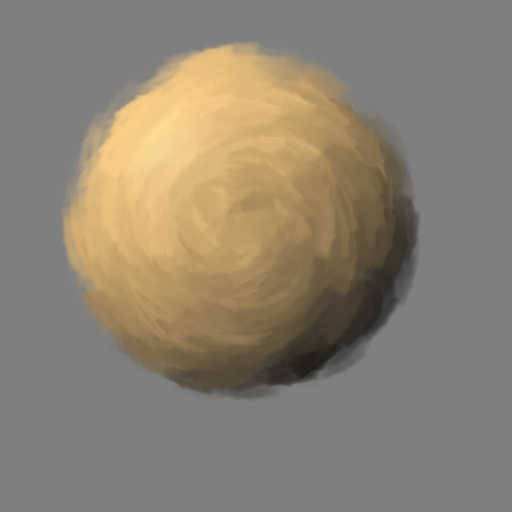
\includegraphics[width=80mm, height=80mm]{Resultats/painting1/final.png}
    \end{center}
    \caption{Example of painting with brushes with our method.}
    \label{final_brushes}
\end{figure}

In order to make an image made like a painter we use an image of a paint strokes (like the fourth in the figure \ref{splat_examples}), we do not need too much splat displayed so the frequency of the procedural noise does not have to be very high but a threshold high/medium, the size of the splats depend of the 3d model but usually we use large splat. For the alpha blending it depends on the effect wanted, in our case, we mixed many splats. And for the orientation usually the artists align the strokes with the tangents but it works well if the strokes are horizontal. The figure \ref{final_brushes} shows the final rendered image. \newline

\textbf{Hair rendering}

\begin{figure}[H]
    \begin{center}
    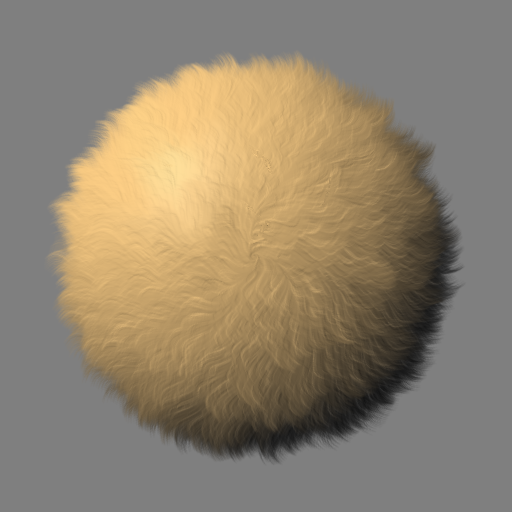
\includegraphics[width=80mm, height=80mm]{Resultats/bouledepoil1/final.png}
    \end{center}
    \caption{Example of hairs rendering with our method.}
    \label{final_hair}
\end{figure}

In order to show that we have the control of the \textit{flatness} impression we tried to create hairs with a 3d aspect like it can be done in digital painting (see figure \ref{final_hair}). To do this we use a splat created mathematically that looks like a hair (the second in the figure \ref{splat_examples}) rotated according to the normals of the object. With the procedural noise that is used to anchor marks, the density can be varied impacting directly the density of hairs in the fur. The size of the splats varies depending on what size you want your hair to be. And for the alpha blending, you do not want to mix too many splats but you do not want to only show the last hairs drawn. The figure \ref{final_hair} shows the final rendered image. \newline

Here there are 3 examples of how we use the method to do some styles but the same styles can be done differently and others styles can be done as well. These 3 examples show what is possible to do with this method and show the control of the \textit{flatness} we have.

\chapter{Practical implementation}




During our research on stylization, we used Gratin \cite{vergne:hal-01254546} which a pipeline rendering software using \textit{OpenGL}. It permits to easily creates rendered images with \textit{GLSL} combining previous images as textures <insert screenshot of gratin>. As we said before every texture used from our contribution can be computed in parallel on GPU including the noises, the fractalization of the noises, the alpha blending and the splatting. Our method use only images as input so it can easily be integrated into every pipeline rendering. For example, if you have a pipeline rendering with \textit{path tracing} to compute the color of your scene you can use this rendered image as color input of our method without re-compute it.\newline

\begin{figure}[H]
    \begin{center}
    \fbox{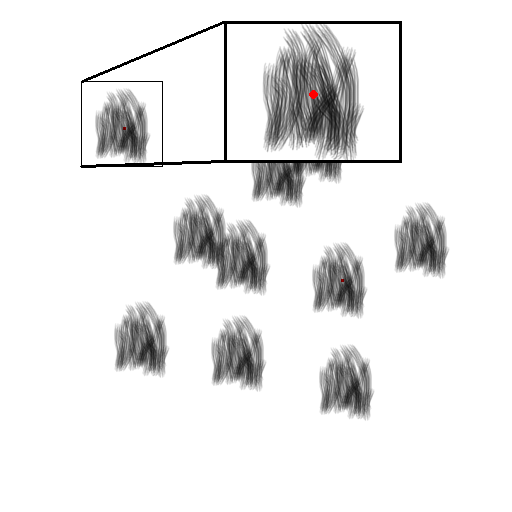
\includegraphics[width=60mm, height=60mm]{images/splatting/splatting4.png}}
    \end{center}
    \caption{Splatting principle: red dots are the anchor points and the splat is centered and anchored to this point.}
    \label{splatting_principle}
\end{figure}

For the splatting step, we draw on each pixel of the screen a square centered on the current pixel (see figure \ref{splatting_principle}). Every square is treated independently on the GPU before in the \textit{vertex shader} which manipulate the 4 vertices of the square which permits the resizing of the splat and permits the rotation of the splat. After this step of resizing and rotation, we pass in the \textit{fragment shader} which manipulate all pixels of splat. It is in this step that we will decide if we display the splat or not thanks to the procedural texture previously computed. \newline

\begin{figure}[H]
    \begin{center}
    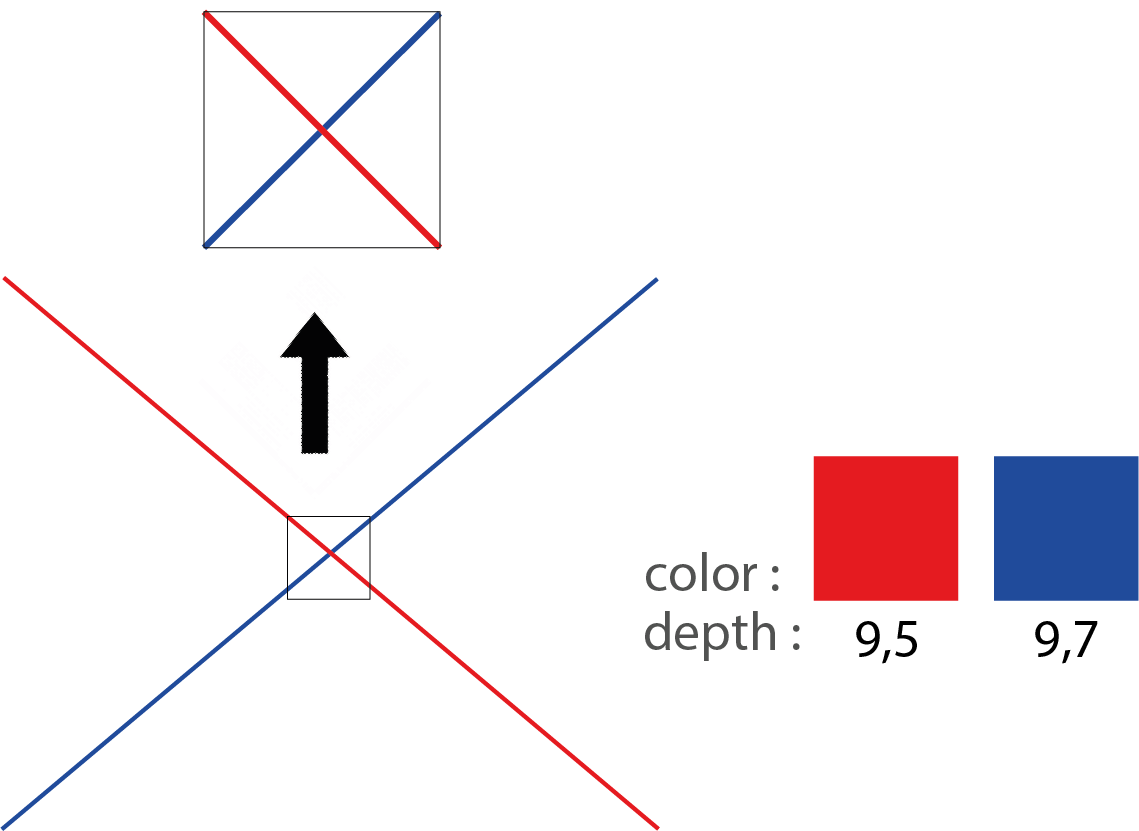
\includegraphics[scale=0.3]{images/splatting/order_independant_transparency.png}
    \end{center}
    \caption{Example of usage of the order independant transparency.}
    \label{order}
\end{figure}



In this \textit{fragment shader}, we prepare the technique of \textit{order-independent transparency} \cite{Munstermann} that consists a structure that permit to know the order of the splats depending on the depth. We create in real time for each pixel of the screen a linked list on the GPU in order to sort the pixels contained in the splat. Thanks to this, we can apply a fonction of alpha blending that take account the position of the splat, their color, their opacity. In our example in the figure \ref{splatting_principle}, we have some splats that cover others splats. How do we know which one is in front of the other if we treat them independently? For example, if there is a pixel where splat covers another one, we construct an array with 2 elements composed of color and a depth so we can know which one is in front of the other one (see example in the figure \ref{order}). We apply the same technique but in our case we have a lot of splats that cover others and as depth to put in this array we use the depth corresponding to vertex of the stylized object where the splat is anchored (the red dots in the figure \ref{splatting_principle} correspond to a vertex of the 3d objects). \newline

After creating these array, we will in the last pass treat each pixel of the screen independently and (still on GPU) decide which color has to be displayed. In order to do this, we sort the array corresponding to the current pixel according to the depth. And finally, we apply our algorithm of alpha blending (the same as the mode "over" in Overcoat \cite{schmid_overcoat:_2011}):

\lstdefinestyle{customc}{
  belowcaptionskip=1\baselineskip,
  breaklines=true,
  frame=L,
  xleftmargin=\parindent,
  language=C,
  showstringspaces=false,
  basicstyle=\footnotesize\ttfamily,
  keywordstyle=\bfseries\color{green!40!black},
  commentstyle=\itshape\color{purple!40!black},
  identifierstyle=\color{blue},
  stringstyle=\color{orange},
}


\lstset{escapechar=@,style=customc}

\begin{lstlisting}
vec4 over(in vec4 c1,in vec4 c2) {
    float a = (c1.a+(1.-c1.a)*c2.a);
    return vec4((c1.rgb*c1.a + c2.rgb*(1.-c1.a)*c2.a)/a,a);
}

vec4 alpha_blending(vec4 colorArray[], int count, vec4 backgroundColor, float gammaBlend){
    // colorArray is the list of color sorted: colorArray[0] correspond to the farest
    // count correspond to the number of splat that we will take account during the blending
    // backgroundColor is the color of the background our image
    // gammaBlend is a user parameter that will increase the transparency of the displayed color

    vec4 finalColor = vec4(0,0,0,0);

    for(int i=count-1; i>=0; i--) {
        vec4 currentColor = colorArray[i];
        finalColor = over(finalColor,vec4(currentColor.rgb,clamp(pow(currentColor.a,1./gammaBlend),0.,1.)));
    }

    return over(finalColor,backgroundColor);
}
\end{lstlisting}

After this algorithm we have the color to display in the current pixel of the image/screen.

% algo fractalization ????

% antialiasing

\chapter{Results and performance}

\begin{figure}
    \begin{center}
    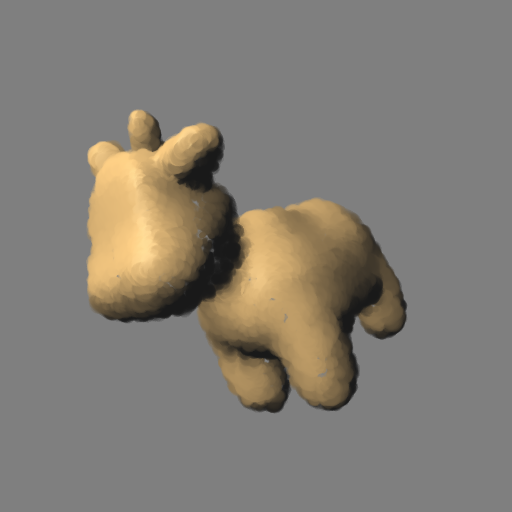
\includegraphics[width=70mm, height=70mm]{Resultats/spotPoint/final.png}
    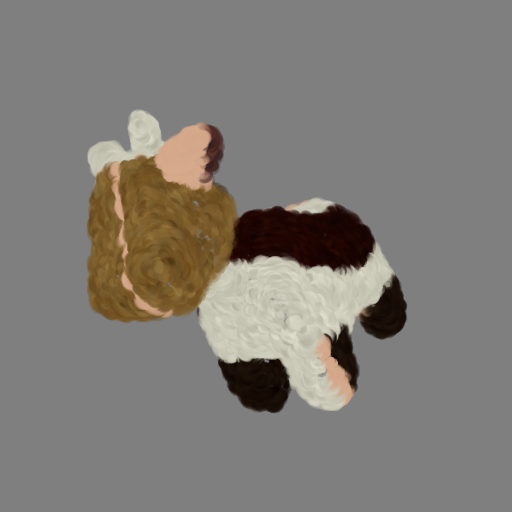
\includegraphics[width=70mm, height=70mm]{Resultats/spotPoint/final2.png}
    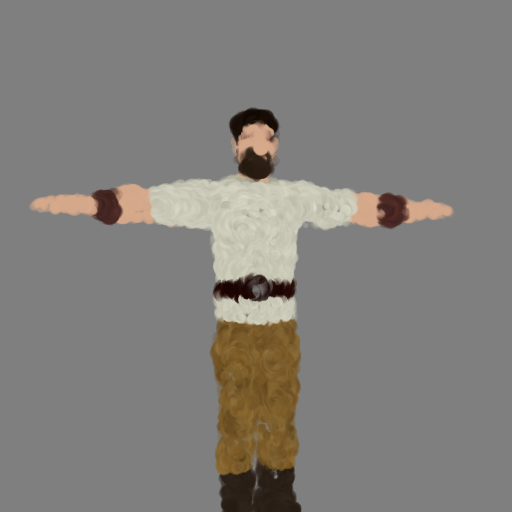
\includegraphics[width=70mm, height=70mm]{Resultats/pointCharacter/final.png}
    \end{center}
    \caption{Results of pointillism.}
    \label{results_point}
\end{figure}

\begin{figure}
    \begin{center}
    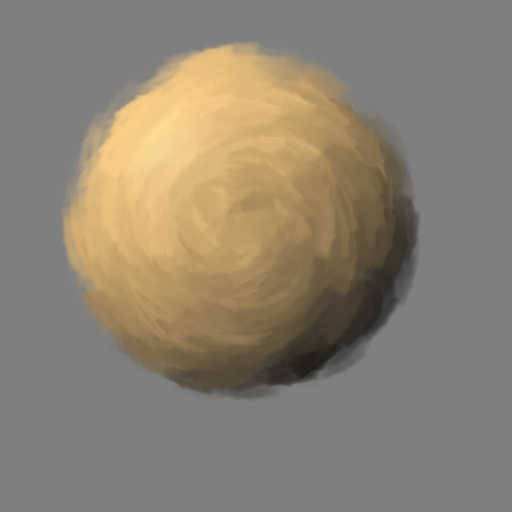
\includegraphics[width=70mm, height=70mm]{Resultats/painting1/final.png}
    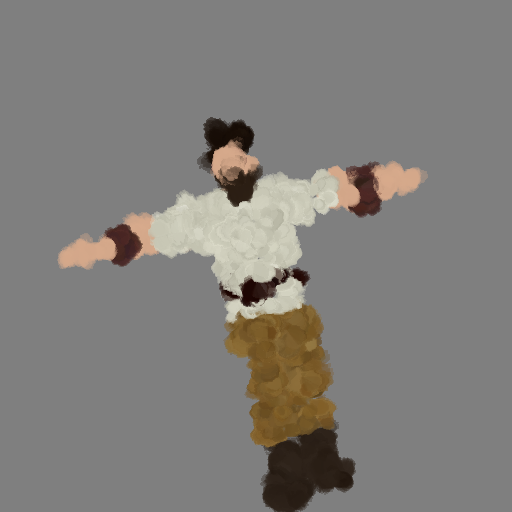
\includegraphics[width=70mm, height=70mm]{Resultats/paintChar/final.png}
    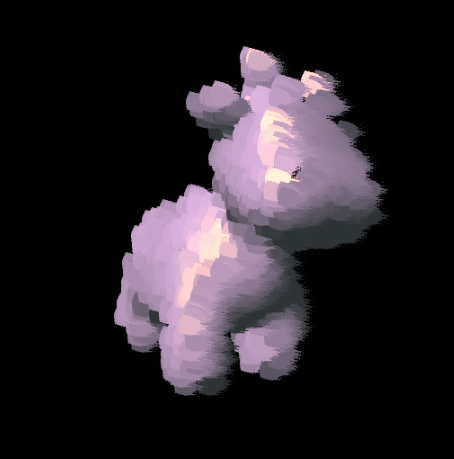
\includegraphics[width=70mm, height=70mm]{Resultats/spotPaint.png}
    \end{center}
    \caption{Results of brush painting.}
    \label{results_paint}
\end{figure}

\begin{figure}
    \begin{center}
    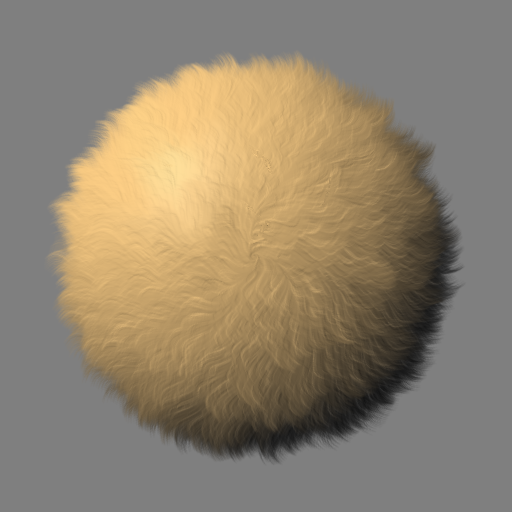
\includegraphics[width=70mm, height=70mm]{Resultats/bouledepoil1/final.png}
    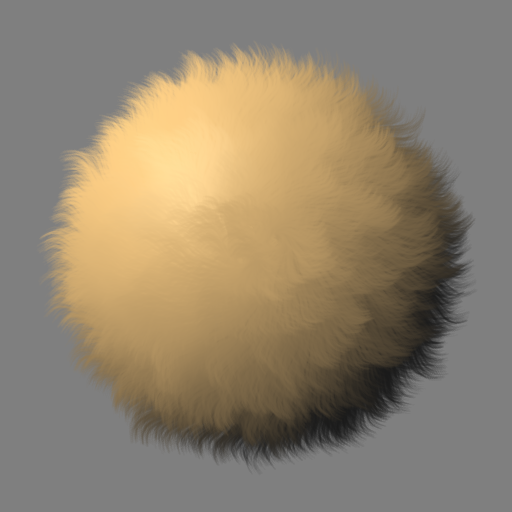
\includegraphics[width=70mm, height=70mm]{Resultats/bouledepoil2/final.png}
    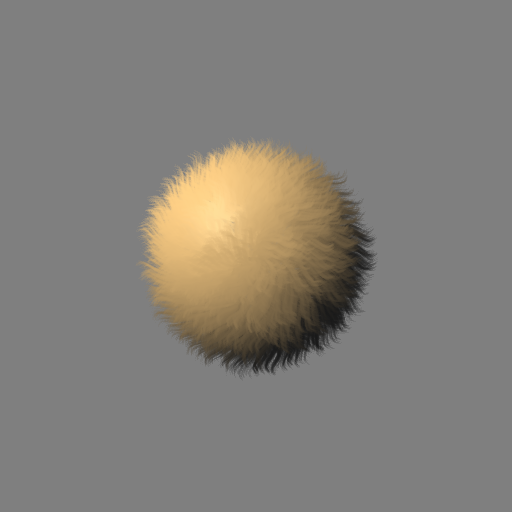
\includegraphics[width=70mm, height=70mm]{Resultats/bouledepoilFractalized/final.png}
    \end{center}
    \caption{Results of hairs rendering.}
    \label{results_hairs}
\end{figure}


Here there are some results of our method of stylization. The figure \ref{results_point} show some rendering with a point as mark and with differents color and models. We use the dot splat (the first in the figure \ref{splat_examples}) with a small size in order to keep a good level of details. In the figure \ref{results_paint} we tried to stylized as painted with brushes so we used brushe stroke as splat. In the figure \ref{results_hairs}, we tried to render hairs with our technique we a simple hair as splat. We rotated it according to the normals and to increase the realism we changed the size of the splat depending of a procedural noise to have in some areas of the object smaller splat and in some others areas bigger splat. In our work, we did not focused on the color of rendered color because it depends on the 3d model and because our solution tend to be integrate in more complex pipeline rendering where the color is computed before.\newline

\textbf{Animations}

During our analysis of the state of the art, we talked about what happened if the camera moves. We made some videos to show the results of our solution with an animated camera. The videos are in the Maxime's website (\href{http://www.maximeisnel.fr/procedural-stylization/}{http://www.maximeisnel.fr/procedural-stylization/}). It is difficult to create a good \textit{flatness} effect while moving, the animations of the brush painting is a good example at each frame we have something that has good \textit{flatness} but during the motion we can see problem of \textit{temporal continuity}. This due to the alpha blending and also mainly due to the size of the splat because they are big and so to improve \textit{temporal continuity} we have to make to splat disappear/appear more slowly in order resolve some popping effect of the splats. As you can see in the animations of hairs rendering the splats are smaller so we don't have this problem of \textit{temporal continuity}. \newline


\textbf{Performance}

Our pipeline is implemented as a set of (non-optimized) OpenGL fragment shader in the Gratin software (\cite{vergne:hal-01254546}). Its performance is affected by the number of sampling during the creation of the procedural noises to minimize aliasing problem (popping effects). But the pipeline is mainly affected by the splatting step and the algorithm of order-independent transparency because in order to stylize the whole object we draw a lot of splat on the image so we have many splat cover others and then in order to know the order of them depending on the depth we sort with a \textit{bubble sort} an array that contains at most 300 elements (arbitrary limits fixed depending on the GPU used) for each pixel of the final image. In other words, the performance depends on how many splats are drawn and their size, if the size of splat is big the splats will cover more splats that if their size is small and the complexity will be higher. For the animation of brush painting (present in Maxime's website) with 300 frames with a resolution of 512x512 pixels, it takes approximately 4 minutes with an Nvidia GeForce RTX 2070 graphics card to render.






%%%% results
% several example with differents splats
% use noise to change the size of the splats in the object
% use tangents/normals map to rotate the splats
% differents shading



%%%% PERF
% nom de la carte
% resolution de l'image
% non-optimized

%\chapter{Conclusion}





\subsection{Futur works}

%\appendix \chapter{Appendix} 

Appendix goes here...
%=========================================================


%=========================================================
\backmatter

\bibliographystyle{plain} % plain-fr si rapport en français
\bibliography{proceduralBib,customBib}

%\cleardoublepage % Goes to an odd page
%\pagestyle{empty} % no page number
%~\newpage % goes to a new even page

\end{document}
